\documentclass{article}
\usepackage{graphicx}
\usepackage{caption}
\usepackage{subcaption}
\usepackage{url}

\usepackage{amsmath}

\newcommand{\code}[1]{\texttt{#1}}
\renewcommand\refname{7  \hspace{4 mm}References}

\begin{document}

\title{CS 867: Displaying Multiple Time Series}
\date{December 16, 2013}
\author{Carmen St.\ Jean}

\maketitle

\section{Introduction}

Time-oriented data might be one of the most common forms of data, used in numerous fields such as medicine, economics, ecology, engineering, and meteorology.  Typically, time series are visualized using line charts, which appear frequently in newspapers, textbooks, and academic papers.  However, it can be difficult to display many concurrent time series at once in an understandable manner using a line chart.  Therefore, we have introduced a new visualization technique called a stack graph, which we propose may be suitable for showing many time series---i.e., fifteen---at once.  To test the merits of our creation, we have evaluated the stacked graph against two existing methods---small multiples and horizon graphs.

\subsection{Background}

Since it was first introduced by William Playfair in 1786 \cite{playfair1786}, the line chart has been a popular choice for displaying temporal data.  However, it has its limitations when it comes to multiple time series.  To be plotted on a single chart, each time series must be distinctly colored and/or patterned; as the number of time series increases, it becomes more difficult to make each series visually distinct.  Even if each time series are designed uniquely, it may be difficult to distinguish two time series which have similar vales and overlap frequently.

\begin{figure}
        \centering
        \begin{subfigure}[b]{0.4\textwidth}
                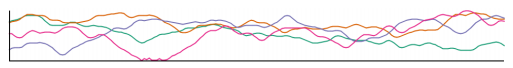
\includegraphics[width=\textwidth]{figures/ts_simplelinegraph.eps}
                \caption{A simple line graph.}
                \label{fig:ts_simple}
        \end{subfigure}
        \begin{subfigure}[b]{0.4\textwidth}
                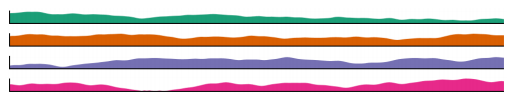
\includegraphics[width=\textwidth]{figures/ts_smallmultiples.eps}
                \caption{Small multiples.}
                \label{fig:ts_smmult}
        \end{subfigure}
        \\
        \begin{subfigure}[b]{0.4\textwidth}
                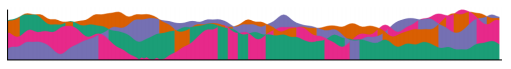
\includegraphics[width=\textwidth]{figures/ts_braidedgraph.eps}
                \caption{A braided graph.}
                \label{fig:ts_braid}
        \end{subfigure}
        \begin{subfigure}[b]{0.4\textwidth}
                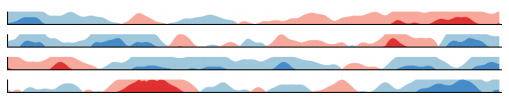
\includegraphics[width=\textwidth]{figures/ts_horizongraphs.eps}
                \caption{Horizon graphs.}
                \label{fig:ts_horizon}
        \end{subfigure}
        \caption{Four possible methods for visualizing multiple time series \cite{javed2010}.}
        \label{fig:ts_compare}
\end{figure}

Recognizing the limitations of the line chart for many time series leads to a question: what is a suitable alternative?  Javed et al.\ set out to answer this question with their evaluation that compared the line chart, as in Figure~\ref{fig:ts_simple}, with three alternative techniques  \cite{javed2010}.  The first alternative, called ``small multiples'' simply places each time series on its own line chart, shown in Figure~\ref{fig:ts_smmult}.  The screen space must be split with this approach, which leads to less resolution in the vertical direction.  Therefore, Javed et al.\ introduced a shared space approach called the ``braided graph'' seen in Figure~\ref{fig:ts_braid}, which attempts to be easier to read than a line chart by coloring the areas underneath the curves.  Additionally, Saito et al.'s horizon graph, as in Figure~\ref{fig:ts_horizon}, was included in the evaluation \cite{saito2005}.

\begin{figure}
        \centering
        \begin{subfigure}[b]{0.5\textwidth}
                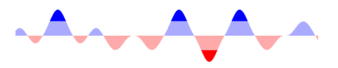
\includegraphics[width=\textwidth]{figures/construction1.eps}
                \caption{The line chart is divided into evenly-spaced bands, which are colored shades of blue in the upper-half and shades of red in the lower-half.}
                \label{fig:construction1}
        \end{subfigure}
        \\ 
        \begin{subfigure}[b]{0.5\textwidth}
                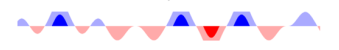
\includegraphics[width=\textwidth]{figures/construction2.eps}
                \caption{The bands of similar colors are layered together.}
                \label{fig:construction2}
        \end{subfigure}
        \\
        \begin{subfigure}[b]{0.5\textwidth}
                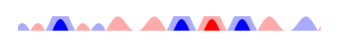
\includegraphics[width=\textwidth]{figures/construction3.eps}
                \caption{The red bands are mirrored.}
                \label{fig:construction3}
        \end{subfigure}
        \caption{Steps for constructing a horizon graph \cite{heer2009}.}
        \label{fig:hg_construction}
\end{figure}

Saito et al.\ designed horizon graphs to increase the amount of data that can be displayed without increasing graph size \cite{saito2005}.  To construct a horizon graph, some ``mid-line'' must be defined; it could represent zero or it could be the average of the global minimum and global maximum values in the dataset.  The areas between the mid-line and the data values are filled in, as in Figure~\ref{fig:construction1}, with blue for areas above the mid-line and red for areas below the mid-line.  The data is then further divided into evenly spaced bands, with the color of the band darkening as distance from the mid-line increases.  Next, these bands are offset to align with the mid-line, as in Figure~\ref{fig:construction2}.  Finally, the red bands are mirrored.  The result is the vertical resolution can be increased by a factor of four, as in Figure~\ref{fig:hg_construction}, or even more if more bands are used.

Javed et al.\ evaluated these four techniques illustrated in Figure~\ref{fig:ts_compare} by having participants complete three tasks on randomly-generated data:
\begin{enumerate}
	\item \textbf{Maximum:} for a given time point, identify the time series with the highest value
	\item \textbf{Slope:} for the entire time period, find the time series with the highest increase
	\item \textbf{Discrimination:} at a time point specific to each series, determine which series has the highest values
\end{enumerate}
In addition to chart type, their study varied the number of time series (2, 4, and 8) and the total chart height (48, 96, and 192 pixels).  They found that the simple line chart and the braided graph were best suited for the maximum task, while the small multiples and horizon graphs were better for the slope and discrimination tasks.  In general, they concluded that simple line charts and small multiples were generally more robust than horizon graphs and their newly introduced braided graphs. Additionally, they found that decreases in chart size did not affect completion time, but did decrease accuracy.  Lastly, as the number of concurrent time series increased, accuracy decreased and completion time increased. 

\section{Approach}

Javed et al.'s approach considered only eight concurrent time series at most, when it is not unusual for many more to appear together in practice.  Therefore, we determined to conduct a similar study but with fifteen concurrent time series.  This number of time series makes simple line charts impractical, so they were not included in our evaluation.  Additionally, we decided to exclude braided graphs because they did not prove to be particularly effective in Javed et al.'s evaluation.  Instead, we have introduced stack graphs, illustrated in Figure~\ref{fig:stackedGraph}, to compare with small multiples and line graphs.  

\begin{figure}[h]
	\centering
	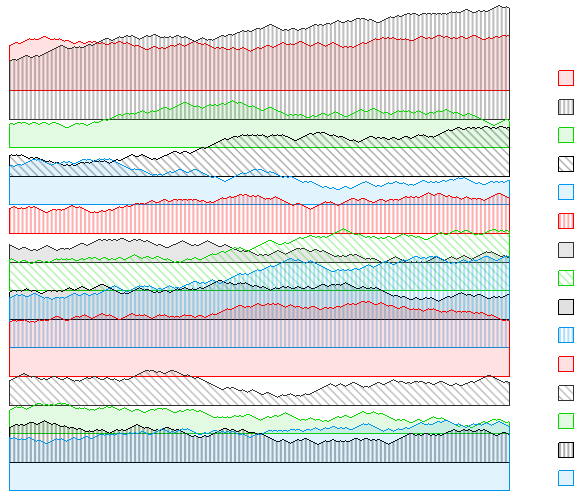
\includegraphics[width=6.5cm]{figures/stacked-new.eps}
	\caption{Fifteen time series represented with stack graphs.}
	\label{fig:stackedGraph}
\end{figure}

Stack graphs are called so because each time series is vertically-offset from the preceding time series, resulting in a stacked appearance.  An $x$-axis and a $y$-axis are drawn for each chart, though the latter is aligned for all charts.  We chose to use an offset of one-fourth of the individial chart height, which means that, at any point, a chart may overlap three other charts.  Therefore, we chose to fill the areas under each time series with semi-transparent, alternating colors and textures that were designed to have maximum see-through.  Our textures are solid, striped, and slanted stripes, while our colors are red, green, blue, and black. The purpose of the stacked graph is to increase the amount of space each chart occupies without increasing space overall.

\begin{figure}[h]
	\centering
	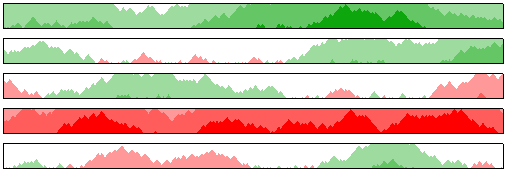
\includegraphics[width=6.5cm]{figures/horizon-new.eps}
	\caption{Five horizon graphs using green for values above the mid-line.}
	\label{fig:newHorizon}
\end{figure}

We have also proposed a different color scheme for the horizon graph, shown in Figure~\ref{fig:newHorizon}, because it can be difficult to remember the meaning of the traditional colors.  If one thinks of a temperature color scale, then red is associated with higher values and blue with lower values, which is the opposite of their intended meanings for horizon graphs.  Users already require instruction and practice to interpret the bands properly, so it would be helpful for them if the colors were less ambiguous.  Therefore, we have replaced blue with green, shown in Figure~\ref{fig:newHorizon}, so that perhaps users will be reminded of the usual financial meanings for these colors: green for above some threshold and red for below it.

\subsection{Display}

All experimentation was conducted on a standard Dell desktop computer with a 20-inch monitor set to 1280 by 1024 pixels resolution.  The portion of the display where the time series were drawn occupied 500 by 515 pixels (approximately 5 by 5.25 inches).  Participants sat so their eyes were approximately 18 inches from the screen.

\subsection{Procedure}

The evaluation consisted of ten trials for each task on each visualization type.  This made for a total of 60 trials per participant.  A trial showed fifteen time series, from which the user selected an answer.  Each time series had a small box drawn next to it, as shown in Figure~\ref{fig:stackedGraph}, which the participant clicked to submit a response.  Response times and correctness of response were recorded.

\subsection{Tasks}

Both tasks involved selecting one time series out of set of fifteen.  The two tasks used were based on the tasks by Javed et al. \cite{javed2010}:
\begin{enumerate}
\item \textbf{Maximum:} We asked the user to identify the time series with the highest value at a given point in time that was marked on all time series.  The time was randomly chosen for each trial so it was no closer than 10\% from the beginning or end of the chart.
\item \textbf{Slope:} Two times were marked on all time series.  The user was instructed to identify the time series which increased the most from the first marked time to the second marked time.  As with the maximum task, these times were randomly chosen so that they were no closer than 10\% from the beginning or the end of the chart.  Furthermore, the distance between the two times was designed to be at least 25\% the width of the chart.
\end{enumerate}

The discrimination task from the Javed et al. study \cite{javed2010} was omitted because it seemed unrelated to ways which time series are read in reality.  Typically, users are concerned with how time series compare at the same point in time or across the same time range, not different times unique to each series.

\subsection{Conditions}

The condition that varied in our study was the visualization type.  Our fifteen time series were represented in one of the following ways:

\begin{itemize}
\item \textbf{Small multiples:} one line chart per time series, with the area between the values and the $x$-axis filled. The same $y$-axis scale was used across all charts.  Each chart was 500 by 26 pixels.
\item \textbf{Horizon graphs:} one three-band horizon graph per time series using the red-green color scheme.  The baseline was set to the average of the global minimum and global maximum values of all time series.  The same $y$-axis scale was used across all charts.  Each chart was 500 by 26 pixels.
\item \textbf{Stack graphs:}  one semi-transparent line chart per time series, with the area between the values and the $x$-axis filled with a texture. Each chart starts at one-fourth up the height of the previous chart. The same $y$-axis scale was used across all charts.  Each chart was 500 by 115 pixels.
\end{itemize}

\subsection{Subjects}

Four volunteers were used as subjects.  All four were graduate students in Computer Science at the University of New Hampshire.  Their vision was either 20-20 vision or corrected to 20-20 with glasses.

\bibliographystyle{plain}

\bibliography{sources}

\end{document}
